\part{Aspect technique}
\label{technique}

\section{Base de données}
\label{sec:technique/bdd}

\subsection{Notre choix de base de données}
\label{subsec:technique/bdd/choix}
\par
Le nombre de mots générés étant très grand, pour faciliter leur exploitation, le choix a été fait d'utiliser un \textbf{système de gestion de base de données} (SGBD). Car même si les résultats sont enregistrés dans des fichiers textes, parcourir et classer des centaines de fichiers et des milliers de lignes de texte est fastidieux et demanderait de coder de nombreux algorithmes, que les SGBD intègrent nativement. De plus, en cas d'évolution ou de changements dans les critères de classements des mots, la solution fichier n'offre aucune flexibilité.
\par
Quant au choix du SGBD, il s'est orienté vers \textbf{PostgreSQL}, un SGDB relationnel respectant la norme SQL, en raison de sa légèreté, de sa licence libre (PostgreSQL License) et de sa facilité d'installation et d'utilisation avec C++.

\subsection{Architecture de la base de données}
\label{subsec:technique/bdd/architecture}
\par
L'architecture de la base de données a été pensée pour \textbf{optimiser le temps de réponse aux requêtes et l'espace occupé}. En effet, on parle de dizaines de millions de mots à enregistrer.
\par
Pour optimiser le temps d'exécution des requêtes, le nombre de colonnes de la table contenant les mots a été réduit au minimum, de sorte qu'il ne reste que les mots et les clés étrangères. Le lien entre les données se fait à l'aide d'unions, l'une des opérations les plus optimisées sur les SGBD relationnels \cite{BROU2012}.

\begin{figure}[!h]
\centering
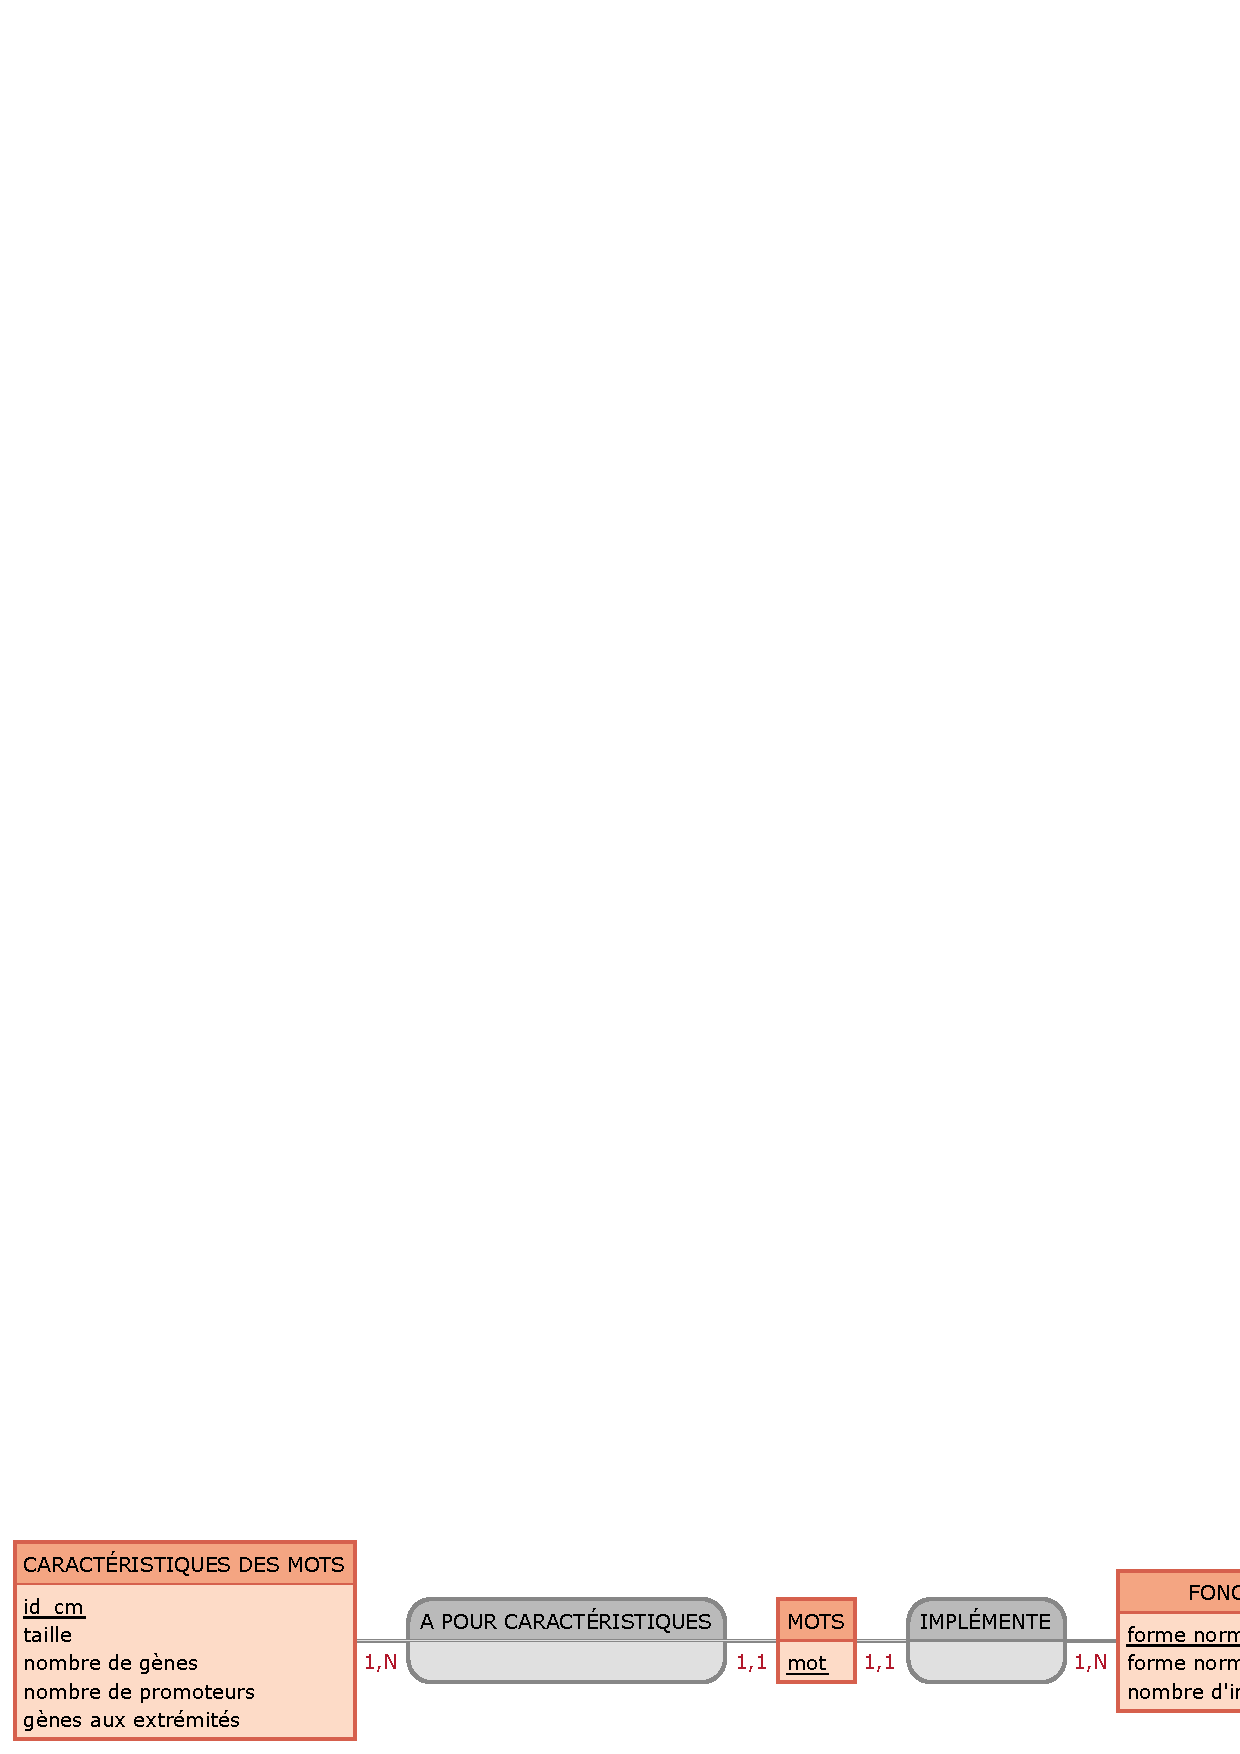
\includegraphics[scale=0.65]{images/MEA_BDD}
\caption{\label{fig:technique/bdd/architecture/1} Modèle entité-association de la base de données}
\end{figure}
\begin{figure}[!h]
\centering
\begin{tabular}{rl}
Caractéristiques des mots & (\underline{id\_cm}, taille, nombre de gènes, nombre de promoteurs, gènes aux extrémités)\\ 
Mots & (\underline{mot}, \textsl{id\_cm}, \textsl{forme normale disjonctive})\\
Fonctions logiques & (\underline{forme normale disjonctive}, forme normale disjonctive, nombre d'inputs)\\
\end{tabular}
\caption{\label{fig:technique/bdd/architecture/2} Modèle relationnel de la base de données}
\end{figure}

\subsection{Utilisation de la base de données}
\label{subsec:technique/bdd/utilisation}
\par
Lors de l'utilisation de notre programme pour trouver les mots qui implémentent une fonction logique, on effectue une requête qui \textbf{classe les mots suivant leur nombre de gènes puis leur taille en nombre de bases}, conformément au souhait exprimé lors d'une consultation avec \bsc{Mme. Guiziou}, la commanditaire du projet.\\

\exx{Avec la fonction logique $A$ :\\
\GR \SF{0} \PF \SR{0} ~est préférable à \GR \SF{0} \TR \SF{0} \PR ~car il est plus court.\\
\PF \GR \SF{0} \TF \TR \SF{0} \PR ~est préférable à \GR \SF{0} \GF \PF \SR{0} ~car il n'a qu'un gène.}

\par
De plus, l'utilisation d'une base de donnée permet de la questionner avec des requêtes personnalisées selon les besoins de l'utilisateur.
\par
Le portage d'une partie du code en PHP nous a également permis de mettre en place \textbf{un site web} offrant un accès instantané, pratique, et graphique à l'ensemble des mots générés, triés par fonction logique et classés. Le site supporte également la recherche d'informations directement sur les mots ou fonctions logiques voulus. Il est accessible à l'annexe \ref{sec:annexes/git}.

\section{Le programme Genetix}
\label{sec:technique/genetix}

\subsection{Nos choix techniques}
\label{subsec:technique/genetix/choix}
\par
Le programme a été codé en \textbf{C++}. C'est un langage objet maîtrisé par les membres du groupe, et sa puissance, sa flexibilité, et sa compatibilité multi-plateforme ont été des atouts au projet. Il fut utilisé dans sa version 11 puis 14 afin de profiter des dernières améliorations en matière de parallélisation, lambdas-fonctions, et pointeurs intelligents.
\par
Nous nous en sommes servis avec les bibliothèques \textbf{Boost}, pour sa gestion des options, des ensemble de bits dynamiques et des fichiers, et \textbf{Pqxx}, le driver C++ de PostgreSQL. Toutes les bibliothèques utilisées sont \textbf{compatibles multi-OS}.
\par
Enfin, notre code source est agrémenté de commentaires formatés pour \textbf{Doxygen}, un générateur de documentation.

\subsection{Utilisation du programme Genetix}
\label{subsec:technique/genetix/utilisation}
\par
Le programme Genetix s'exécute par ligne de commande et son aide détaillée peut être obtenue par \texttt{genetix -h}. Il permet d'effectuer toutes les tâches relatives au projet. On peut obtenir des informations sur des mots : symétrique, table de vérité, fonction logique implémentée sous forme minimale ; sur des fonctions logiques : table de vérité, forme minimale, 10 meilleurs mots qui l'implémentent ; ou encore comparer les deux. Il est également possible de lancer la génération si l'on souhaite se créer la base de données de mots.
\par
Un tableau récapitulatif des options du programme est disponible en annexe \ref{sec:annexes/options}.